\appendix

\section{Proofs}\label{app:proofs}

\subsection{Proof of Theorem \ref{thm1} and Theorem \ref{thm2}}
Sequential and advanced composition are standard; see~\cite{dwork2014algorithmic}.

\subsection{Proof of Theorem \ref{thm4} (Sensitivity of $H$)}
\begin{proof}
Let $ z $ and $ z '$ be the random variables associated with the two histograms (m dimension) calculated by two adjacent datasets $ D $ and $ D' $, respectively. Both data sets have n records, but only one record is different.

Let $ z_c = (c_1, c_2, \dots, c_m) $ and $ z_c '= (c'_1, c'_2, \dots, c'_m) $ denote the $ z $ and $ z' $ attributes, respectively Histogram of m values. Entropy is calculated on the probability distribution represented by the histogram.

Note that the histograms of the adjacent datasets $ D $ and $ D '$ considered can only differ in two positions. If there is no difference in any position, then the lemma is generally $ (\ Delta H = 0) $. In other words, without loss of generality, there are $ j_1 $ and $ j_2 $ of which $ (j_1 \neq j_2) $, such that $ c '_{j_1} = c_{j_1} + 1 $ and $ c' _{j_2 } = c_{j_2} -1 $.

In addition, $ n-1 \geq c_{j_1} \geq 0 $, which means $ n \geq c_{j_1} ' \geq 1 $, and $ n \geq c_ {j_2} \geq 1 $, which Means $ n-1 \geq c'_{j_2} \geq 0 $. In addition, for $ i \neq j_1, j_2 $, we have $ c'_i = c_i $, and:

\begin{eqnarray}
\sum^m_{i=1} c_i = \sum^m_{i=1} c'_i =n
\end{eqnarray}

Now here is,
\begin{equation}
\begin{aligned}
H(z) = - \sum^m_{i=1} \frac{c_i}{n} log_2 \frac{c_i}{n} \\
    =  - \frac{1}{n} [\sum^m_{i=1} c_i log_2 c_i - n log_2 n] \\
    = log_2 n - \frac{1}{n} ( c_{j_1} log_2 c_{j_1} + c_{j_2} log_2 c_{j_2}  \\
       + \sum_{i \neq j_1,j_2} c_i log_2 c_i)
\end{aligned}
\end{equation}
Similar are:
\begin{eqnarray}
\begin{aligned}
H(z') = log_2 n - \frac{1}{n} \sum_{i \neq j_1,j_2} c_i log_2 c_i \\
 - \frac{1}{n}[(c_{j_1} + 1)log_2 (c_{j_1} +1) + (c_{j_2} - 1) log_2 (c_{j_2} -1)]
 \end{aligned}
\end{eqnarray}

We have $ \Delta_H = max_{c_{j_1}, c_{j_2}} | H (z)-H (z') | $, but for the sake of brevity, we have omitted the maximum value and analysed this number and  The relationship between the values of $ {c_{j_1}} $ and $ {c_{j_2}} $ to show the performance of the lemma in each case.
Observations are:
	\begin{eqnarray}
	\begin{aligned}
	\Delta_H =  |H(z) - H(z')|  \\
			= \frac{1}{n}|c_{j_1}log_2 {c_{j_1}} - (c_{j_1}+1) log_2 (c_{j_1}+1) \\
			 + c_{j_2}log_2 c_{j_2} - (c_{j_2} -1)log_2(c_{j_2}-1)|
			  \end{aligned}
	\end{eqnarray}	
	In the first case: $ c_{j_1} = 0 $ we have
	  	\begin{eqnarray}
	  \Delta_H = \frac{1}{n}|c_{j_2}\log_2 {c_{j_2}}  - (c_{j_2}-1) \log_2 (c_{j_2}-1)|
	  \end{eqnarray}
	 Obviously, if $ c_{j_2} = 1 $, then $ \Delta H = 0 $ and the bound holds. So suppose $ c_{j_2}> 1 $. We have:
	  	  	\begin{eqnarray}
	  	  	\begin{aligned}	
	  \Delta_H = \frac{1}{n}|c_{j_2}log_2 {c_{j_2}} - (c_{j_2}-1) log_2 (c_{j_2}-1)| \\
	  =  \frac{1}{n} |c_{j_2}log_2(\frac{c_{j_2}}{c_{j_2}-1}) + log_2(c_{j_2}-1)| \\
	  \leq \frac{1}{n} |c_{j_2}log_2(\frac{c_{j_2}}{c_{j_2}-1})| + \frac{1}{n} log_2 (c_{j_2}-1)| \\
	  \leq  \frac{1}{n} log_2(n-1) + \frac{1}{n} |(a+1) log_2 (1+ \frac{1}{a})|
	  			  \end{aligned}
	  \end{eqnarray}
	Inside, $(a + 1) log_2(1 +\frac{1}{a})\leq 2$. It is conclusion:$\Delta_H \leq \frac{1}{n}(2 + log_2 n)$.
	 
	 
	 In the second case: $ c_ {j_1} = 1 $ we have
	 \begin{eqnarray}
	 \Delta_H = \frac{1}{n}|c_{j_1}log_2 {c_{j_1}}  - (c_{j_1}+1) log_2 (c_{j_1}+1)|
	 \end{eqnarray}
	 Again, if $ c_{j_1} = 0 $, then the bound holds. So suppose $ c_ {j_1}> 0 $. We have:
	 \begin{eqnarray}
	 \begin{aligned}	
	 \Delta_H = \frac{1}{n}|c_{j_1}log_2 {c_{j_1}} - (c_{j_1}+1) log_2 (c_{j_1}+1)| \\
	 =  \frac{1}{n} |c_{j_1}log_2(\frac{c_{j_1}}{c_{j_1}+1}) - log_2(c_{j_1}+1)| \\
	 \leq \frac{log_2 n }{n} + \frac{1}{n}| c_{j_1} log_2 (\frac{c_{j_1}}{c_{j_1}+1})| \\
	 = \frac{log_2 n }{n}  + \frac{1}{n} c_{j_1} log_2 (\frac{c_{j_1}+1}{c_{j_1}}) \\
	  = \frac{log_2 n }{n}  + \frac{1}{n} c_{j_1} log_2 (1+ \frac{1}{c_{j_1}}) 
	 \end{aligned}
	 \end{eqnarray}
	 Using the L'H\^{o}pital rule, we have $c_{j_1} \log_2(1 + \frac{1}{c_{j_1}}) \leq \frac{1}{\ln 2}$. Thus $\Delta H \leq \frac{1}{n}(2+ \frac{1}{\ln 2} + 2\log_2 n)$.
	 
	 
	 In the third case:$c_{j_1} \geq 1 ,c_{j_2} \geq 1 $ we have:
	 	 \begin{eqnarray}
	 \begin{aligned}	
	 \Delta_H = \frac{1}{n}|c_{j_1}log_2 {c_{j_1}} - (c_{j_1}+1) log_2 (c_{j_1}+1) \\ + c_{j_2} log_2 c_{j_2} - (c_{j_2}-1)log_2 (c_{j_2} -1 ) | \\
	 \leq \frac{1}{n}|c_{j_1}log_2 {c_{j_1}} - (c_{j_1}+1) log_2 (c_{j_1}+1) \\
	 + \frac{1}{n}| c_{j_2}log_2 c_{j_2} - (c_{j_2} -1)log_2(c_{j_2}-1)|
	 \end{aligned}
	 \end{eqnarray}
	 
	 It can be seen here that for Case 1 and Case 2, these two terms are bounded. So put them together, we conclude $\Delta_H \leq \frac{1}{n} (2+ \frac{1}{ln 2} + 2 log_2 n)$.
\end{proof}



\subsection{Proof of Lemma \ref{lemma:2yinU}}
\begin{proof}

Fix y and follow the description of mechanism 1, we have:
\begin{equation}
\begin{aligned}
\mathbb{P}\mathrm{r}\{\mathcal{F}(D^*)=y\} = \sum_{s \in D^*} \mathbb{P}\mathrm{r}\{\mathrm{seed}\;s,\, (D^*,s,y)\;\mathrm{pass\;test}\} \\
=\dfrac{1}{|D^*|} \sum_{s\in D^*} \bigl[p_s(y)\,\mathbb{P}\mathrm{r}\{(D^*,s,y)\;\mathrm{pass\;test}\}\bigr]
\end{aligned}
\end{equation}
\end{proof}


\subsection{Proof of Lemma \ref{lemma4:djparittion} and Corollary \ref{corollary:ismallthan0}}


\begin{proof}
	Fix and let j be the partition where d 'falls into.

    For part (a), note that for $ i \neq j $, we have $ C_i (D, y) = C_i (D ', y) $. So $ q (D, i, y) = q (D ', i, y) $.\\
    For part (b), we have:
			\begin{equation}
	\begin{aligned}
	q(D, j, y) = pt(D, j, y) \sum_{s\in C_j(D,y)} 	p_s(y)  \\
	< pt(D, j, y) [ \sum_{s\in C_j(D,y)} p_s(y) + p_{d'}(y)  ] \\
	= pt(D, j, y) \sum_{s\in C_j(D',y)} p_s(y) \\
	\leq  pt(D', j, y) \sum_{s\in C_j(D',y)} p_s(y) \\
	= q(D', j, y)   
		\end{aligned}
	\end{equation}
Assume that $pd'(y)> 0$ and $pt(D',j,y)\leq pt(D,j,y)$(Lemma~\ref{lemma4:djparittion})	
	
Now, if $| C_j(D,y)| <t$,so:
			\begin{equation}
\begin{aligned}
q(D', j, y) = pt(D', j, y) \sum_{s\in C_j(D,y)} 	p_s(y)  \\
\leq e^{-\varepsilon_0(k-t)}\sum_{s\in C_j(D,y)} 	p_s(y) \\
\leq t e^{-\varepsilon_0(k-t)} ,  
\end{aligned}
\end{equation}

For any d, given$| C_j(D',y)|\leq t $and $pd(y)\leq1$. Here, the first inequality is derived from the following facts:$pt(D',j,y)= \mathbb{P}r \{L\geq k-| C_j(D',y)|\}\leq \mathbb{P}r\{L \geq k-t\} = \frac{1}{2} e^{-\varepsilon_0(k-t)}$.

If$| C_j(D,y)| \geq t$,We have:
			\begin{equation}
\begin{aligned}
q(D', j, y) = pt(D', j, y) \sum_{s\in C_j(D,y)} 	p_s(y)  \\
=  pt(D', j, y) [\sum_{s\in C_j(D,y)} 	p_s(y) +p_{d'}(y)]  \\
\leq e^{\varepsilon_0}pt(D, j, y) [\sum_{s\in C_j(D,y)} 	p_s(y) +p_{d'}(y)]  \\ 
\leq e^{\varepsilon_0} [ 1+\frac{\gamma}{t}]pt(D, j, y) \sum_{s\in C_j(D,y)} 	p_s(y)   \\ 
\leq e^{\varepsilon_0} q(D, j, y),
\end{aligned}
\end{equation}

Given Lemma \ref{lemma4:djparittion} and any$s\in C_j(D,y)$. And we have $pd'(y)\leq \gamma t Ps\in C_j(D,y)ps(y)$ the true is $p_{d'}(y)\leq \frac{\gamma}{t} \sum_{s\in C_j (D,j)} ps(y)$.
\end{proof}

\subsection{Proof of Lemma \ref{lemma5:random1}}


\begin{proof}
	Repair an arbitrary synthetic record$y\in \mathcal{U}$ And any data set D and$| D | \geq k$. Let $D'=D\bigcup\{d'\}$ for any $d'\in \mathcal{U}$is established. From lemma \ref{lemma:2yinU}. Applied to D, we have:$\mathbb{P}r \{F(D)= y\} = | \frac{1}{D} | \sum_{i \leq 0} q(D,i,y)$. In addition, from inference \ref{corollary:ismallthan0}, We have all i$q(D,i,y)\leq q(D',i,y)$. thereby:
	
	\begin{equation}
	\begin{aligned}
	\mathbb{P}r\{ \mathcal{F}(D) = y\}  = \frac{1}{|D|}\sum_{i\geq 0} q(D,i,y)\}  \\
	\leq \frac{1}{|D|}\sum_{i\geq 0} q(D',i,y)\}  \\
	= \frac{|D'|}{|D|} \mathbb{P}r\{ \mathcal{F}(D') = y\} \\
	\leq (1+ \frac{1}{k}) \mathbb{P}r\{ \mathcal{F}(D') = y\}
	\end{aligned}
	\end{equation}
	Due (by assumption)$\gamma > 1$ and $1\geq t\geq k$,We have:$\frac{1}{k} \leq \frac{1}{t}$,and so$1 + \frac{1}{k} <1 +\frac{\gamma}{t} \leq e^{\varepsilon_0} (1 +\frac{\gamma}{t})=e^\varepsilon$. This shows the first part.
	
	For the second part, use lemma \ref{lemma:2yinU} apply to D ', and let j be the number of divisions of d', that is, $ j = I_ {d '} (y) $. We have:
		\begin{equation}
	\begin{aligned}
	\mathbb{P}r\{ \mathcal{F}(D) = y\}  = \frac{1}{|D|}\sum_{i\geq 0} q(D,i,y)\}  \\
	= \frac{1}{|D|}[\sum_{i\geq 0:i\neq j} q(D',i,y)+q(D',j,y)\} ]  \\
	= \frac{1}{|D|}\sum_{i\geq 0:i\neq j} q(D,i,y)+\frac{q(D',j,y)}{|D'|}\}  
	\end{aligned}
	\end{equation}
	The final equality follows the lemma \ref{lemma4:djparittion} part (a).
	
	Using the lemma \ref{lemma4:djparittion} part (b), we get two cases.
	
	
	Case 1:$|C_j(D,y)| <t$. We have:
		\begin{equation}
\begin{aligned}
\mathbb{P}r\{ \mathcal{F}(D') = y\}  = \frac{1}{|D|}\sum_{i\geq 0:i\neq j} q(D,i,y)+\frac{q(D',j,y)}{|D'|} \\
\leq \frac{1}{|D'|} \sum_{i\geq 0:i\neq j} q(D,i,y)+ \delta (D',j,y) \\
\leq \frac{1}{|D'|} \sum_{i\geq 0} q(D,i,y)+ \delta (D',j,y) \\
=  \frac{|D|}{|D'|}\mathbb{P}r\{ \mathcal{F}(D) = y\} + \delta (D',j,y) \\
\leq \mathbb{P}r \{ \mathcal{F} (D) = y\} + \delta
\end{aligned}
\end{equation}

Among them $\delta (D',j,y) = \frac{1}{|D'|} e^{-\varepsilon_0(k-t)}\sum_{s\in C_j(D',y)}p_s(y)$.

Case 2:$|C_j(D,y)| \geq t$. We have:
			\begin{equation}
	\begin{aligned}
	\mathbb{P}r\{ \mathcal{F}(D') = y\}  \\
	= \frac{1}{|D'|}[\sum_{i\geq 0:i\neq j} q(D,i,y)+q(D',j,y)] \\
	\leq \frac{1}{|D'|}[\sum_{i\geq 0:i\neq j} q(D,i,y)+e^{\varepsilon_0}[1+\frac{\gamma}{t}]q(D,j,y)] \\
	\leq e^{\varepsilon_0} [1+\frac{\gamma}{t}]\frac{1}{|D'|}\sum_{i\geq 0:i\neq j} q(D,i,y)\\
	= e^{\varepsilon_0} [1+\frac{\gamma}{t}]\frac{|D|}{|D'|} \mathbb{P}r\{ \mathcal{F}(D) = y\}\\
	\leq e^{\varepsilon_0}  \mathbb{P}r\{ \mathcal{F}(D) = y\}
	\end{aligned}
	\end{equation}
	For $\varepsilon=  \varepsilon_0+ ln(1 +\frac{\gamma}{t} )$ we have $\frac{|D|}{|D'|} <1$, so $\mathbb{P}r\{ \mathcal{F}(D') = y\} \leq e^{\varepsilon} \mathbb{P}r\{ \mathcal{F}(D) = y\}$.
	
	Let   $\delta(D',d',y)=\delta(D',I_{d'}(y),y)$,
	Proof end.
\end{proof}

\subsection{Proof of Lemma \ref{lemma:neighboringdatasets} (Neighboring datasets)}\label{Lemma:proofofneighbor}
\begin{proof}
	There are two cases: $ i = I_d '(y) $ or $ i \neq I_d' (y) $. If $ i = I_d '(y) $, then $ d' $ falls into partition i, so $ C_i (D', y) = C_i (D, y) \bigcup d' \} $. We have:
		\begin{equation}
	\begin{aligned}
	pt(D, i, y) = \mathbb{P}r \{ L \geq k - |C_i(D',y)|\}  \\
	\leq e^{\varepsilon_0} \mathbb{P}r \{ L \geq k - |C_i(D',y)|+1\} \\
	= e^{\varepsilon_0}  \mathbb{P}r \{ L \geq k - |C_i(D',y)|\} = e^{\varepsilon_0} pt(D,i,y)
	\end{aligned}
	\end{equation}
	In addition, we have this: $pt(D', i, y) > pt(D, i, y)$ 
	
	Otherwise, if $ i \neq I_{d '} (y) $, then $ C_i (D', y) = C_i (D, y) $ and so on:
		\begin{equation}
	\begin{aligned}
	pt(D', i, y) = \mathbb{P}r \{ L \geq k - |C_i(D,y)|\}  =  pt(D,i,y) 
	\end{aligned}
	\end{equation}
	Putting it together will produce results.
	
\end{proof}

\subsection{Proof of Theorem \ref{thm5} (Differential privacy of $\mathcal{F}$)}\label{thm5:proof}

\begin{proof}

First consider the condition of $D_1 = D$ and $D_2 = D'$.Applied lemma \ref{lemma5:random1},we got:


Using $|D|$fix dataset $|D|\geq k$for any records $d' \in \mathcal{U}$. Let $D'=D \bigcup \{d'\}$.$\mathcal{F}$is the range of $\mathcal{U}$,so all result is subset of $\mathcal{U}$ a none empty subset. Using $Y \leq \mathcal{U} $ fix an arbitrary$Y\in \phi $.

We will prove that no matter $D_1 = D$ and $D_2 = D'$, or $D_1 = D'$ and $D_2 = D$, we have $\mathbb{P}\mathrm{r}\{\mathcal{F}(D_1)\in Y\} \leq e^\varepsilon\,\mathbb{P}\mathrm{r}\{\mathcal{F}(D_2)\in Y\} + \delta$.


First consider the condition of $D_1 = D$ and $D_2 = D'$. Using lemma \ref{lemma5:random1},we can get:
    \begin{equation}
\begin{aligned}
\mathbb{P}\mathrm{r}\{\mathcal{F}(D)\in Y\} = \sum_{y\in Y} \mathbb{P}\mathrm{r}\{\mathcal{F}(D)=y\}  \\
\leq \sum_{y\in Y} e^{\varepsilon}\,\mathbb{P}\mathrm{r}\{\mathcal{F}(D')=y\}  \\
= e^{\varepsilon}\,\mathbb{P}\mathrm{r}\{\mathcal{F}(D')\in Y\}  
\end{aligned}
\end{equation}
Now consider condition of $D_1 = D'$ and $D_2 = D$. Definition $c(d',y)= | C_I d'(y)(D,y)|$. Given d', We can divide Y in $y\in Y$. In this way, the d 'falling partition has at least t partitions, and the partition partition is smaller than t. which is $Y = Y_{t-}\bigcup Y_{t+}$,$Y_{t-}= \{y:y\in Y,c(d',y)<t\}$ and $Y_{t+}= \{y:y\in Y,c(d',y)\geq t\}$. We have:
        {\footnotesize
    \begin{equation}
\begin{aligned}
\mathbb{P}r\{ \mathcal{F}(D') \in Y\}  &= \sum_{ y\in Y} \mathbb{P}r\{ \mathcal{F}(D') = y\}  \\
&\leq \sum_{ y\in Y_{t+}} e^{\varepsilon}\mathbb{P}r\{ \mathcal{F}(D) = y\} \\
&\quad + \sum_{ y\in Y_{t-}} \bigl[ e^{\varepsilon}\mathbb{P}r\{ \mathcal{F}(D) = y\} + \delta (D', I_{d'}(y),y) \bigr]  \\
&= e^{\varepsilon}\sum_{ y\in Y} \mathbb{P}r\{ \mathcal{F}(D) = y\} + \sum_{ y\in Y_{t-}} \delta (D', d',y) \\
&= e^{\varepsilon} \mathbb{P}r\{ \mathcal{F}(D) \in Y\} + \sum_{ y\in Y_{t-}} \delta (D', d',y). 	
\end{aligned}
\end{equation}
    }
Where the inequality is based on$ y\in Y_{t-} $(Lemma \ref{lemma5:random1} in Case 1)and $ y\in Y_{t+} $(Lemma \ref{lemma5:random1}the proof of condition 2),Let introduce lemma \ref{lemma4:djparittion} and ~\ref{lemma5:random1} condition with in each y.

Thus $\sum_{ y\in Y_{t-}} \delta (D', d',y) \leq e^{-\varepsilon_0(k-t)}$, so the mechanism satisfies $(\varepsilon,\delta)$-DP with $\delta = e^{-\varepsilon_0(k-t)}$. For this definition$C(D', d',y)=C_{I_{d'(y)}}(D',y)$. We have: 
    \begin{equation}
\begin{aligned}
\sum_{ y\in Y_{t-}} \delta (D', d',y) 	 = \sum_{ y\in Y_{t-}} \frac{e^{-\varepsilon_0(k-t)}}{|D'|}\sum_{ s\in C(D', d',y)} p_s(y)  \\
    =	\frac{e^{-\varepsilon_0(k-t)}}{|D'|} \sum_{s \in D'} \sum_{y\in Y_{t-}} \mathbb{I}_{I_{d'} (y) = I_S(y)}   p_s(y) \\
        \leq e^{-\varepsilon_0(k-t)}
\end{aligned}
\end{equation}
For all $s\in D'$, we have $\sum_{y\in Y_{t-}} \mathbb{I}_{I_{d'}(y) =I_s(y)}   p_s(y) \leq \sum_{y\in \mathcal{U}} p_s(y) \leq  1$
Where $I_{I_d '(y)}$ is the space of $d' (y)$ in the $II$ domain. Its spatial intersection $I_s (y) P_s (y)$ is less than the upper limit of $P_s (y)$.
	
\end{proof}

\section{Figure and table data descriptions}\label{app:figdata}
Table~\ref{tab:figures_theory} summarizes, for each figure, the data shown and the part of the theory it supports.
\begin{table*}[t]
\centering
\caption{Summary: each figure's data description and the theory it supports.}
\label{tab:figures_theory}
\begin{tabular}{clp{5.2cm}}
\hline
\textbf{Figure} & \textbf{Data} & \textbf{Theory supported} \\
\hline
\ref{fig:generalpic} & Pass rate vs.\ $\gamma$; curves for $k \in \{10,20,30,50\}$ & Theorem~\ref{thm5} (mechanism $\mathcal{F}$ is $(\varepsilon,\delta)$-DP); privacy test. \\
\ref{fig:GaussianKernel1} & Original vs.\ private RKHS mean; $\rho = 10^{-6}, 0.001, 0.1$ & Wiener kernel mechanism; $\rho$ utility--privacy tradeoff. \\
\ref{fig:epsilon_utility} & PSNR, MAE vs.\ $\varepsilon$; Laplace \& Gaussian & $(\varepsilon,\delta)$-DP utility--privacy tradeoff. \\
\ref{fig:entropy_bound} & $\Delta_H$ bound vs.\ $n$ & Theorem~\ref{thm4} (entropy sensitivity). \\
\ref{fig:metrics_comparison} & PSNR, MAE, SSIM at $\varepsilon = 0.5, 1, 2$ & Laplace vs.\ Gaussian. \\
\ref{fig:csv_entropy} & Histogram \& entropy (Table~\ref{tab:csv_entropy}) & Theorem~\ref{thm4}; Laplace histogram release. \\
\ref{fig:csv_entropy_multi} & Multi-dataset entropy (Table~\ref{tab:csv_entropy_multi}) & Generality of entropy--DP framework across domains. \\
\ref{fig:fig8} & (See caption) & (See caption) \\
\hline
\end{tabular}
\end{table*}

\section{Additional experimental result}\label{app:extrafig}
\begin{figure}[t]
	\centering
	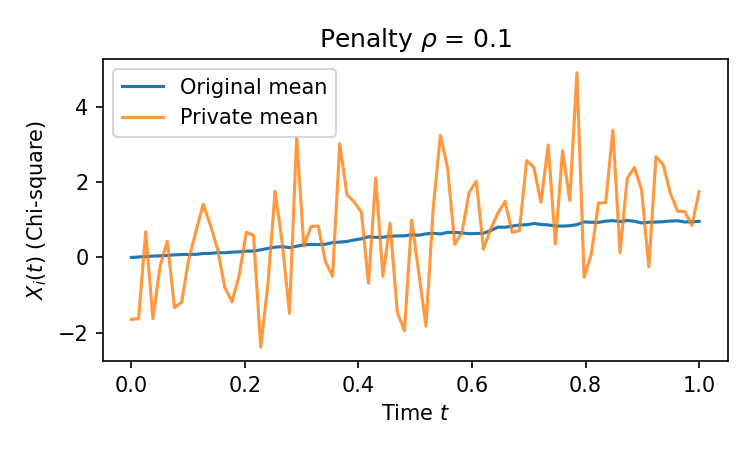
\includegraphics[width=\columnwidth]{fig/fig8.png}
	\caption{Additional experiment (see text).}\label{fig:fig8}
\end{figure}
Figure~\ref{fig:fig8} provides a further experimental result. It can be used to illustrate an extended comparison (e.g., different datasets, parameter sweeps, or ablation) and is included for completeness.

\section{Full multi-dataset validation results}\label{app:multidata}
\begin{table*}[t!]
\centering
\caption{Multi-dataset real-data validation: same entropy+DP pipeline on seven datasets ($\varepsilon=1$, 30 bins; $n$ capped at 100k where applicable).}
\label{tab:csv_entropy_multi}
\begin{tabular}{lrrrrrr}
\hline
Dataset (column) & $n$ & bins & $\varepsilon$ & $H_{\mathrm{orig}}$ & $H_{\mathrm{noisy}}$ & $\Delta_H$ bound \\
\hline
y\_amazon-google-large ($y$) & 100000 & 30 & 1.0 & 3.0279 & 3.0286 & 0.00037 \\
house-prices-train (SalePrice) & 1460 & 30 & 1.0 & 3.4873 & 3.5155 & 0.01676 \\
home-credit-application-train (AMT\_INCOME\_TOTAL) & 100000 & 30 & 1.0 & 0.0004 & 0.0034 & 0.00037 \\
tabular-feature-engineering ($y_1$) & 10000 & 30 & 1.0 & 4.6645 & 4.6640 & 0.00300 \\
r\_diff\_train ($y_1$) & 10000 & 30 & 1.0 & 0.0237 & 0.0459 & 0.00300 \\
pow\_train ($y_1$) & 10000 & 30 & 1.0 & 4.7066 & 4.7065 & 0.00300 \\
unemployment\_data (UNRATE) & 601 & 30 & 1.0 & 4.0457 & 4.0894 & 0.03645 \\
\hline
\end{tabular}
\end{table*}

\begin{figure*}[t!]
	\centering
	\subfigure[Amazon-Google reviews ($y$).]{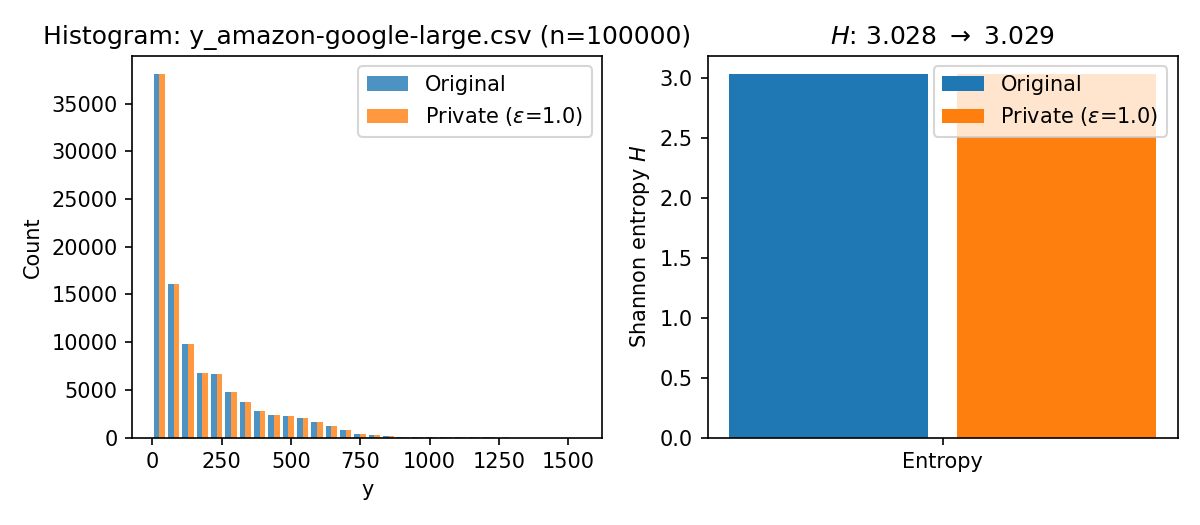
\includegraphics[width=0.48\textwidth]{fig/fig_csv_entropy_y_amazon-google-large.png}}
	\hfill
	\subfigure[House prices (SalePrice).]{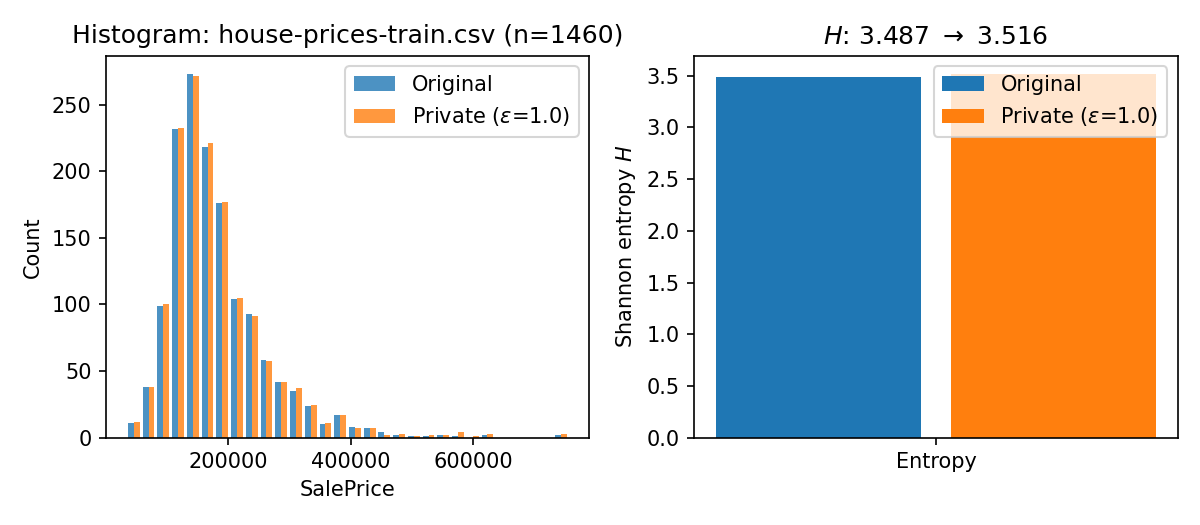
\includegraphics[width=0.48\textwidth]{fig/fig_csv_entropy_house-prices-train.png}}\\
	\subfigure[Tabular feature engineering ($y_1$).]{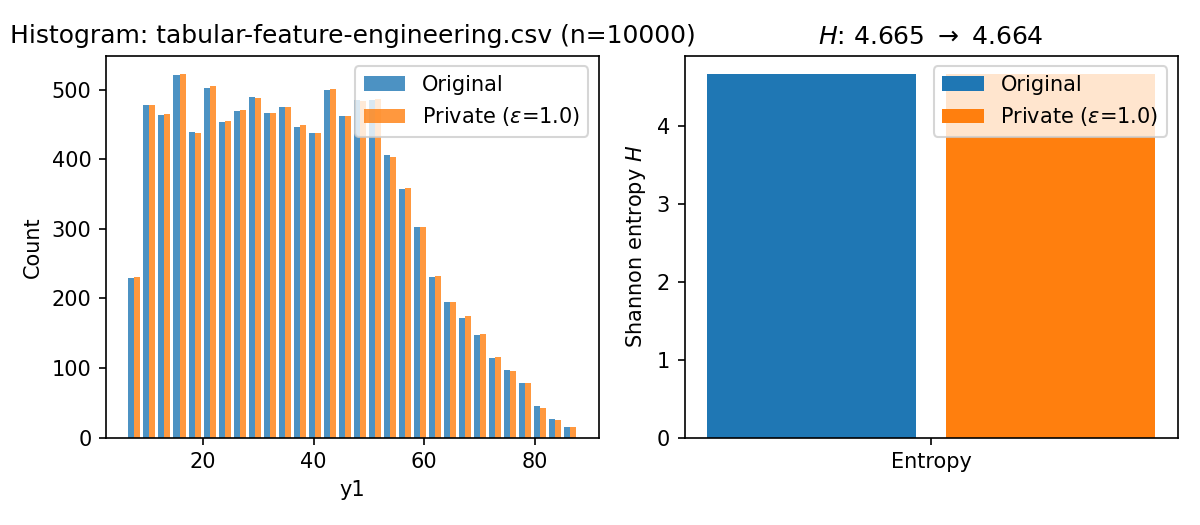
\includegraphics[width=0.48\textwidth]{fig/fig_csv_entropy_tabular-feature-engineering.png}}
	\hfill
	\subfigure[U.S. unemployment (UNRATE).]{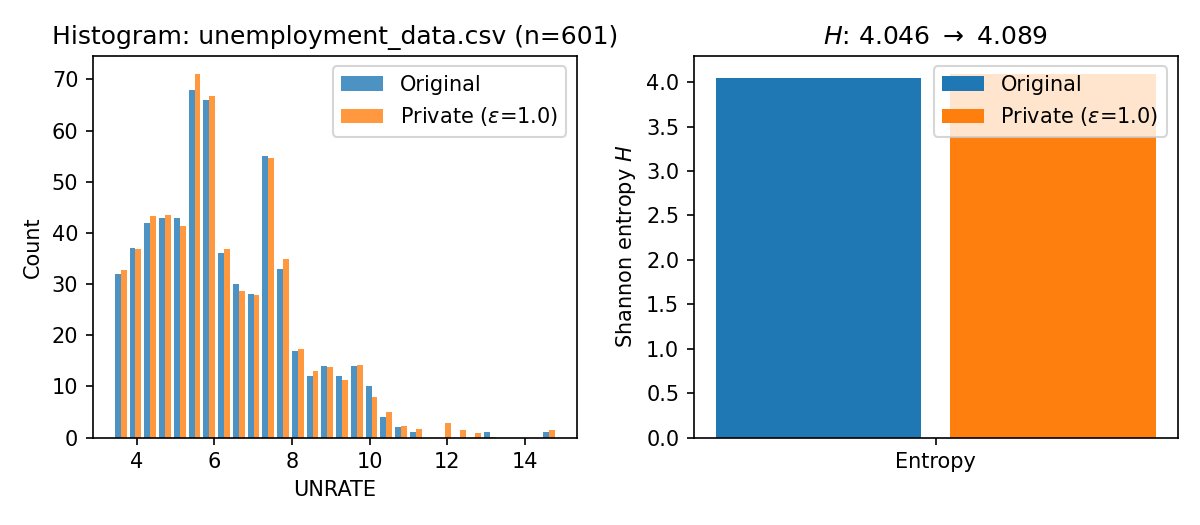
\includegraphics[width=0.48\textwidth]{fig/fig_csv_entropy_unemployment_data.png}}
	\caption{Multi-dataset validation: histogram and entropy (original vs.\ $\varepsilon$-DP) on four representative public datasets. Same mechanism and Theorem~\ref{thm4} bound; full table in Table~\ref{tab:csv_entropy_multi}.}\label{fig:csv_entropy_multi}
\end{figure*}
